\documentclass{article}

% if you need to pass options to natbib, use, e.g.:
\PassOptionsToPackage{numbers, compress}{natbib}
% before loading nips_2016
%
% to avoid loading the natbib package, add option nonatbib:
% \usepackage[nonatbib]{nips_2016}

\usepackage{nips_2016} % TODO: undo final!

% to compile a camera-ready version, add the [final] option, e.g.:
% \usepackage[final]{nips_2016}

\usepackage[utf8]{inputenc} % allow utf-8 input
\usepackage[T1]{fontenc}    % use 8-bit T1 fonts
%\usepackage{hyperref}       % hyperlinks % TODO: include? it seems to blow things up otherwise?
\usepackage{url}            % simple URL typesetting
\usepackage{booktabs}       % professional-quality tables
\usepackage{amsfonts}       % blackboard math symbols
\usepackage{nicefrac}       % compact symbols for 1/2, etc.
\usepackage{microtype}      % microtypography

\title{Data-Efficient Reinforcement Learning in \\ Continuous State-Action POMDPs} % TODO: change title from POMDPs to noisy? or observation noise?

\author{
Rowan Thomas McAllister\\
Department of Engineering\\
Cambridge University\\ % TODO: we can cut out some of this stuff, to make it a bit shorter?
Cambridge, CB2 1PZ\\
\texttt{rtm26@cam.ac.uk} \\
\And
Carl Edward Rasmussen \\
Department of Engineering\\
University of Cambridge\\
Cambridge, CB2 1PZ\\
\texttt{cer54@cam.ac.uk} \\
}

% The \author macro works with any number of authors. There are two commands
% used to separate the names and addresses of multiple authors: \And and \AND.
%
% Using \And between authors leaves it to \LaTeX{} to determine where to break
% the lines. Using \AND forces a linebreak at that point. So, if \LaTeX{}
% puts 3 of 4 authors names on the first line, and the last on the second
% line, try using \AND instead of \And before the third author name.

%\newcommand{\fix}{\marginpar{FIX}}
%\newcommand{\new}{\marginpar{NEW}}

%\nipsfinalcopy % Uncomment for camera-ready version

% My additions
\usepackage{tikz}
\usetikzlibrary{arrows,shapes,backgrounds,patterns,fadings,decorations.pathreplacing,decorations.pathmorphing}
\tikzset{>=stealth'}
\usetikzlibrary{arrows}
\usepackage{pgfplots}
\pgfplotsset{compat=1.9}
\usetikzlibrary{positioning}
\usepackage{amsmath}
\usepackage{amssymb}
\usepackage{algorithm}
\usepackage{algorithmic}

%\usepackage{textcomp}
%\usepackage{eulervm}
%\usepackage[T1]{fontenc}
%\usepackage[utf8]{inputenc}

\newcommand{\N}{\mathcal{N}}
\newcommand{\C}{{\mathbb C}}
\newcommand{\E}{{\mathbb E}}
\newcommand{\V}{{\mathbb V}}
\newcommand{\pno}[1]{#1_{t|t-1}}   % Prediction step NOw
\newcommand{\uno}[1]{#1_{t|t}}     % Update step NOw
\newcommand{\unot}[1]{\tilde #1_{t|t}}     % Update step NOw, jointly with control
\newcommand{\pne}[1]{#1_{t+1|t}}   % Prediction step NEw
\newcommand{\pnee}[1]{#1_{t+2|t+1}}   % Prediction step NEwer
\newcommand{\pneT}[1]{#1_{T|T-1}}   % Prediction step NEwest
\newcommand{\une}[1]{#1_{t+1|t+1}}     % Update step NEw
\newcommand{\now}[1]{#1_t}
\newcommand{\nowt}[1]{\tilde #1_t}
\newcommand{\new}[1]{#1_{t+1}}
\newcommand{\neww}[1]{#1_{t+2}}
\newcommand{\newT}[1]{#1_{T}}
\newcommand{\unotMbm}{\uno{\mu}^{\tilde\bm}}
\newcommand{\unotSbm}{\uno{\Sigma}^{\tilde\bm}}
\definecolor{lgrey}{rgb}{0.8,0.8,0.8}
\newcommand{\argmin}[1]{\underset{#1}{\operatorname{arg}\operatorname{min}}\;}
\newcommand{\inv}{^{-1}}
\newcommand{\nnn}{\nonumber \\}
\newcommand{\nn}{\nonumber}
\newcommand{\fx}{f} % dynamics model
\newcommand{\fb}{f} % {f_b} % dynamics model for the prediction remove % currently we'll leave this a f so we don't have to respecify what f_b all means.
\newcommand{\bm}{m} % belief mean
\newcommand{\BM}{M} % random belief mean
\newcommand{\der}{\text{d}} % derivative
\newcommand{\expcost}{\mathcal{E}}
\newcommand{\uw}{\text{vec}} % unwrap operator
\newcommand{\newlinetimesdist}{\hspace{0.3cm}\times\;}
%\definecolor{grey}{rgb}{0.7,0.7,0.7}
%\definecolor{dgrey}{rgb}{0.35,0.35,0.35}
%\newcommand{\blue}[1]{\textcolor{blue}{#1}}
\newcommand{\red}[1]{\textcolor{red}{#1}}
\newcommand{\policyparams}{\psi} % \theta
\newcommand{\pendulumangle}{\theta} %
\newcommand{\gplinear}{\phi} % gp linear function

\newcommand{\note}[1]{}        % OFF

%\allowdisplaybreaks

%\newcommand{\graphA}{graph0.tex}  % OFF
%\newcommand{\graphB}{graph0.tex}  % OFF
\newcommand{\graphA}{graph1.tex} % ON
\newcommand{\graphB}{graph2.tex} % ON

\usepackage{graphicx}
\usepackage{caption}
\usepackage{subcaption}

% \renewcommand{\rmdefault}{psbx}
%\usepackage{textcomp}
%\usepackage{eulervm}
% \setlength{\textwidth}{160mm}
% \setlength{\oddsidemargin}{0mm}
% \setlength{\parindent}{0 mm}
\newcommand{\bff}{{\bf f}}
\newcommand{\bfm}{{\bf m}}
\newcommand{\bfx}{{\bf x}}
\newcommand{\invt}{{^{-\top}}}

% For margins
\setlength{\belowcaptionskip}{-15pt}
\usepackage[small,compact]{titlesec}
\titlespacing{\section}{0pt}{1ex}{0.8ex}
\titlespacing{\subsection}{0pt}{0.5ex}{0ex}
\titlespacing{\subsubsection}{0pt}{0.2ex}{0ex}
\expandafter\def\expandafter\normalsize\expandafter{%
    \normalsize
    \setlength\abovedisplayskip{2pt}
    \setlength\belowdisplayskip{2pt}
    \setlength\abovedisplayshortskip{0pt}
    \setlength\belowdisplayshortskip{0pt}
}
%\renewcommand{\baselinestretch}{0.95}

\begin{document}
\maketitle

\begin{abstract}

We present a data-efficient reinforcement learning
method for continuous state-action systems
under significant observation noise.
%from physical-states to belief-states by considering filtering-dynamics
%in addition to physical-dynamics during policy evaluation.
%Our method extends the highly data-efficient PILCO algorithm.
%We instead predict distributions of \textit{belief}-trajectories,
Data-efficient solutions under small noise exist,
such as PILCO which learns the cartpole swing-up task in 30s.
%A highly data-efficient algorithm applicable to low-noise systems is PILCO.
%achieved unprecedented data-efficiency
%in benchmark systems such as the cartpole swing-up.
PILCO %is a policy search method,
evaluates policies by planning state-trajectories using a dynamics model.
However, PILCO applies policies to the observed state,
therefore planning in \textit{observation}-space.
We extend PILCO with filtering to instead plan in \textit{belief}-space,
consistent partially observable Markov decisions process (POMDP) planning.
%corresponding to a POMDP treatment.
This enables data-efficient learning under significant observation noise,
outperforming more naive methods such as \textit{post-hoc} application of a filter to
policies optimised by the original (unfiltered) PILCO algorithm.
We test our method on the cartpole swing-up task, %  with sensor noise
which involves nonlinear dynamics and requires nonlinear control.
\end{abstract}

\section{Introduction}

The Probabilistic Inference and Learning for COntrol (PILCO) \cite{pilco} framework
is a reinforcement learning algorithm, which uses Gaussian Processes (GPs)
to learn the dynamics in continuous state spaces.
The method has shown to be highly \emph{efficient} in the sense that it can
learn with only very few interactions with the real system.
However, a serious limitation of PILCO is that it assumes that the observation noise level is small.
There are two main reasons which make this assumption necessary.
Firstly,
%1)
the dynamics are learnt from the noisy observations,
but learning the transition model in this way doesn’t correctly account of the noise in the observations.
If the noise is assumed small, then this will be a good approximation to the real transition function.
%
Secondly,
%2)
PILCO uses the noisy observation directly to calculate the action,
which is problematic if the observation noise is substantial.
Imagine a policy controlling an unstable system,
where high gain feed-back is necessary for good performance.
%Feeding the noisy input directly to the high gain controller
%will cause the controller to inject noise into the state.
Observation noise is \textit{amplified} when the
noisy input is fed directly to the high gain controller,
which in turn injects noise back into the state,
creating cycles of increasing variance and instability. %can rapidly destabilise a system.
%soon destabilising the system
%The noise is then
%\textit{amplified} by the high gain,
%which produces large variation in controller output,
%quickly.

In this paper we extend PILCO to address these two shortcomings,
enabling PILCO to be used in situations with substantial observation noise.
The first issue is addressed using the so-called \emph{direct} method for training the transition model,
see section~\ref{sec:direct}. The second problem can be tackled by \emph{filtering} the observations.
One way to look at this is that PILCO does planning in observation space, rather than in belief space.
In this paper we extend PILCO to allow filtering of the state,
by combining the previous state distribution with the dynamics model and the observation using Bayes rule.
Note, that this is easily done when the controller is being applied, but to gain the full benefit,
we have to also take the filter into account when optimising the policy.

PILCO trains its policy through minimising the expected predicted loss when \emph{simulating}
the the system and controller actions. Since the dynamics are not known exactly,
the simulation in PILCO had to simulate \emph{distributions} of possible trajectories
of the physical state of the system. This was achieved using an analytical approximation based on
moment-matching and Gaussian state distributions. In this paper we thus need to augment the simulation
over physical states to include the state of the filter, an \textit{information state} or \textit{belief state}.
This is a bit more complicated as the belief state itself is a probability distribution,
we will now have to simulate distributions over distributions.
This will allow the algorithm both to apply filtering during control but also to anticipate the
effect of filtering during training, thereby learning a better policy.

We will first give a brief outline of related work in section~\ref{sec:relatedwork} and
the original PILCO algorithm in section~\ref{sec:pilco},
including the proposed use of the `direct method' for training dynamics
from noisy observations in section~\ref{sec:direct}.
In section~\ref{sec:bayespilco} will derive the algorithm for POMDP training or planning in belief space.
Note an assumption is that we observe noisy versions of the state variables.
We do not handle more general cases where other unobserved states are also learnt nor
learn any other mapping from the state space to observations other than additive Gaussian noise.
In the final sections we show experimental
results showing that the proposed algorithm handles observation noise better than competing algorithms,
and close with conclusions and discussion.

% \subsection{...}
% Real world control systems rely on imperfect sensors
% to control processes where poor performance often causes real expense.
% Learning to control such systems thus entails:
% 1) an inability to know the state of the system with certainty
% and 2) penalties for data-inefficiency.

% \subsection{Data Efficiency}
% Most reinforcement learning (RL) methods are data-intensive,
% requiring much system interaction before learning good policies
% (e.g. \cite{deepmind-continuous-control}). % TODO: more cites?
% For systems prone to wear and tear, or expensive to operate, data-efficiency is critical.
% Model-based RL methods learn models of the unknown system dynamics.
% They are generally more data-efficient than model-free RL
% because they can generalise from local dynamics knowledge gained and
% propagate otherwise-local value backups globally throughout state-action space
% \cite{atkeson1997,boone1997efficient}.
% %
% Unfortunately, a common problem in model-based RL is model bias.
% Model bias typically arises when
% predictions are based on only a single model
% selected from a large plausible set,
% leaving the RL method susceptible to model error.
% An example is using the maximum a posteriori (MAP) model.
% Any single model from a large plausible set
% is quite possibly the wrong model,
% being just one of the many plausible
% explanations of what generated the observed data.
% And the less data observed, the greater the number of plausible dynamics models.
% When optimising data-efficiency,
% the agent constantly learns and acts in the low-data regime
% where the set of plausible models is vast,
% exacerbating model bias effects.
% This regime undermines traditional trajectory-based control approaches
% which assume model-correctness,
% such as model predictive control or iterative linear quadratic regulators. % TODO: verify?
% Unless model-based RL algorithms consider the complete set of plausible dynamics,
% they will succumb to model-bias,
% counteracting the data-efficiency benefits of using a model.
%
% % Data-efficiency key = probabilistic model!
% PILCO is a model-based RL algorithm which achieved unprecedented data-efficiency in
% learning to control the cartpole swing-up problem
% whilst only scaling linearly with horizon \cite{pilco}.
% The key to PILCO's success is its % (single)
% \textit{probabilistic} dynamics model,
% which makes predictions by marginalising over the complete set of
% plausible dynamics functions. % (given the current data).
% By additionally propagating
% model uncertainty throughout trajectory prediction
% PILCO avoids model bias.
% %
% % TODO: reword below
% As a result, PILCO more likely collects data in
% promising areas of the state space.
% %yielding data-efficient learning.

\section{Related Work}\label{sec:relatedwork}
%\subsection{Sensor Noise}
% %How well a dynamical system can be controlled
% %ultimately depends on how well the system is observed.
% The reality of imperfect, noisy sensors present two issues:
% 1) difficulty in identifying the system dynamics, and
% 2) difficulty in deciding actions when the system state is only partially observed.
% %impairs
% %the control of dynamical systems. % TODO: too obvious?
% Such problems can be framed mathematically by
% partially observable Markov decision processes (POMDPs).
% Solving a POMDP is more complex than its fully observable counterpart, the MDP \cite{pomdp}.
% A common approximation with small-noise POMDPs
% is therefore to ignore noise. This assumes full observability
% by learning and planning in observation space rather than latent state space.
% However, such approximations break under larger noise levels. % TODO: reword? noise dominated settings?
% For example, consider the cartpole system (Figure~\ref{fig:cartpole}).
% Stabilising the pendulum upright requires a controller
% with a large gain associated with
% the pendulum angle.
% This enables the cart to move quickly under the pendulum's centre of gravity
% in response to slight angle variations.
% When incorrectly modelled as an MDP,
% noise associated with reading the pendulum's angle is injected directly into the policy.
% The noise is then
% \textit{amplified} by the high gain,
% which produces large variation in controller output,
% quickly destabilising the system.

% The negative effects of sensor noise can be
% mitigated using an observation model and filtering.
% To \textit{filter} a sequence of sensory outputs is
% to maintain a belief posterior distribution
% over the latent system state
% conditioned on the complete history of previous actions and observations.
Implementing a filter is straightforward
when the system dynamics are \textit{known} and \textit{linear},
referred to as Kalman filtering.
For known nonlinear systems,
the extended Kalman filter (EKF) is often adequate (e.g.\ \cite{van2012efficient}),
as long as the dynamics are \textit{locally linear},
meaning approximately linear within the region covered by the belief distribution. % TODO: too wordy?
Otherwise, the EKF's first order Taylor expansion approximation breaks down.
Greater nonlinearities usually warrant the unscented Kalman filter (UKF)
or particle methods \cite{bayesFilters,particleMethods}.
The UKF uses a deterministic sampling technique to estimate moments.
However, if moments can be computed analytically and exactly,
moment-matching methods are preferred.
Moment-matching using distributions from the exponential family (e.g.\ Gaussians)
is equivalent to optimising the Kullback-Leibler divergence $\text{KL}(p||q)$
between the true distribution $p$ and an approximate
distribution $q$.
In such cases, moment-matching is less susceptible to model bias than the EKF % TODO: reword again?
due to its conservative predictions \cite{deisenroth2013}.
%Of course, a lack of filtering can usually be compensated by purchasing higher quality sensors,
%however, we are interested how to get the best performance from inexpensive, off-the-shelf hardware.
%
% \subsection{Related Work and Our Method}
% TODO Compare against \cite{van2012efficient}
Unfortunately, the literature does
not provide a continuous state-action method that is both data efficient and resistant to noise
when the dynamics are \textit{unknown} and \textit{locally nonlinear}.
Sometimes the dynamics are partially-known, with known functional form yet unknown parameters.
Such `grey-box' problems have the aesthetic solution of incorporating
the unknown dynamics parameters into state,
reducing the learning task into a POMDP planning task \cite{duff2002,webb2014online,ross2008bayesian}.
Finite state-action space tasks can be similarly solved,
e.g.\ only two Dirichlet parameters are required to model the probability of each
of the finitely-many state-action-state transitions \cite{poupart2006}.
However, such solutions are not suitable for continuous-state `black-box' problems with no prior dynamics knowledge.
\note{PILCO fails...}
The original PILCO does not assume any prior dynamics knowledge,
yet assumes full state observability and fails under moderate sensor noise.
One proposed solution is to filter observations during policy execution \cite{deisenroth2013}.
%Filtering during execution does indeed improve performance,
%which we demonstrate later.
However, without also predicting system trajectories w.r.t.\ the filtering process, % TODO: simulation or prediction?
the above method merely optimises policies for unfiltered control, not for filtered control.
The mismatch between unfiltered-prediction and filtered-execution
restricts PILCO's ability to take full advantage of filtering. % TODO: too wordy?
%
\citet{dallaire2009} optimise a policy using a more realistic filtered-prediction.
However, the method neglects model uncertainty by only
using the maximum a posteriori (MAP) model.
Unlike the method of \citet{deisenroth2013} which gives a full probabilistic treatment of the dynamics predictions,
work by \citet{dallaire2009}
is therefore highly susceptible to model error,
hampering data-efficiency.

% We propose the best of both worlds,
% by extending PILCO from MDPs to POMDPs using full probabilistic predictions w.r.t.\ a filtered process.
We instead predict system trajectories using closed loop filtered control precisely because
we execute closed loop filtered control.
The resulting policies are thus optimised for the specific case in which they are used.
Doing so,
our method retains the same data-efficiency properties of PILCO
whilst applicable to tasks with high observation noise.
%For simplicity, we only consider a special case of POMDPs,
%specifically those where the partial observability is in the form of Gaussian noise on the latent state vector.
%
To evaluate our method, we use the benchmark cartpole swing-up task with noisy sensors.
We show realistic and probabilistic prediction (to consider uncertainty)
helps our method outperform aforementioned methods.
%This includes adding a filter post hoc to a controller learned using an unfiltered simulator does better.
%But the real performance gains are when we learn with a filter in the loop.
%
% This paper proceeds by summarising the PILCO framework in greater detail (section~\ref{sec:pilco}),
% which we modify and extend for application to POMDPs (section~\ref{sec:bayespilco}).
% We then compare our method with
% the aforementioned methods in the cartpole swing-up problem
% (section~\ref{sec:experiments}),
% discussing each method's predicted and empirical performance
% (section~\ref{sec:result-and-analysis}).

\section{The PILCO Algorithm}\label{sec:pilco}

\newcommand{\linedefpolicy}{1}
\newcommand{\lineinitpolicy}{2}
\newcommand{\lineexecute}{4}
\newcommand{\linetrain}{5}
\newcommand{\linepredict}{6}
\newcommand{\lineevaluate}{7}
\newcommand{\lineoptimise}{8}

PILCO is a model-based policy-search RL algorithm.
It applies to continuous-state, continuous-action, continuous-observation and
discrete-time control tasks.
A probabilistic dynamics model is used to predict one-step system dynamics
(from one timestep to the next).
This allows PILCO to probabilistically predict multi-step system trajectories
over arbitrary time horizon $T$,
by repeatedly using the predictive dynamics model's output at one timestep,
as the (uncertain) input
in the following timestep.
For tractability PILCO uses moment-matching to keep the latent state distribution Gaussian.
The result is an analytic distribution of state-trajectories,
approximated %as a set of marginal
as a joint Gaussian distribution over $T$ states. % over the state space.
%one per timestep.
The policy is evaluated as the expected total cost of the trajectories.
%with expectation over the trajectory distribution. % and a user-supplied cost function.
Next, the policy is improved using local gradient-based optimisation,
searching over policy-parameter space. %using the aforementioned steps for
A distinct advantage of moment-matched prediction for policy search
instead of particle methods
is smoother policy gradients and less local optima \cite{mchutchon2014}.
Finally, the policy is executed, generating additional data
to re-train the dynamics model.
The whole process then repeats until policy convergence.
%
For the remainder of this section
we discuss, step by step, PILCO summarised by Algorithm~\ref{algo:pilco}.
The user first defines a parametric policy $\pi$ function (Algorithm~\ref{algo:pilco}, line~\linedefpolicy)
and then initialises the policy parameters $\policyparams$ randomly (line~\lineinitpolicy)
since we begin without any data.

\subsection{System Execution Phase}
With a policy now defined, PILCO is ready to \textit{execute} the system (Algorithm~\ref{algo:pilco}, line~\lineexecute).
Let the latent state of the system at time $t$ be \smash{$\now{x}\in\mathbb{R}^D$},
which is noisily observed as \smash{$\now{z}=\now{x}+\now{\epsilon}$},
where \smash{$\now{\epsilon}\stackrel{iid}{\sim}\N(0,\Sigma^\epsilon)$}.
%
The policy $\pi$, parameterised by $\policyparams$,
takes observation $\now{z}$ as input,
and outputs a control action $\now{u}=\pi(\now{z},\policyparams)\in\mathbb{R}^F$.
%
Applying action $\now{u}$ to the dynamical system in state $\now{x}$,
results in a new system state $\new{x}$. %with new state at the following timestep denoted .
%
%This completes the description of system execution,
Repeating until horizon $T$ results in a new single state-trajectory of data.

\subsection{Learning Dynamics} % TODO: define $f$ more mathy...reviewer wanted it defined.
To learn the unknown dynamics (Algorithm~\ref{algo:pilco}, line~\linetrain),
any probabilistic model flexible enough to capture the complexity of the dynamics can be used.
Bayesian nonparametric models
are particularly suited given their resistance to overfitting and underfitting respectively.
Overfitting otherwise leads to model bias,
and underfitting limits the complexity of the system this method can learn to control.
%
In a nonparametric model
no prior dynamics knowledge is required, not even knowledge of
\textit{how complex} the unknown dynamics might be
since the model's complexity grows with the available data.
%
We define the latent dynamics $\fx: \nowt{x} \rightarrow \new{x}$,
where $\nowt{x} \doteq [\now{x}^\top,\now{u}^\top]^\top$.
%
PILCO models the dynamics with $D$ independent Gaussian process (GP)
priors, one for each dynamics output variable:
\smash{$\fx^a: \nowt{x} \rightarrow \new{x}^a$}, where \smash{$a\in[1,D]$} is the $a$'th dynamics output,
and \smash{$\fx^a \sim \mathcal{GP}(\gplinear_a^\top {\tilde x}, k({\tilde x}_i,{\tilde x}_j))$}.
Note we implement PILCO with a linear mean function\footnote{
The original PILCO instead uses a zero mean function, and instead predicts relative changes in state.}
$\gplinear_a^\top \tilde x$.
The covariance function $k$ is squared exponential,
with length scales $\Lambda_a=\text{diag}([l_{a,1}^2,...,l_{a,D+F}^2])$,
and signal variance $s_a^2$:
%\begin{eqnarray}
\smash{$k^a(\tilde x_i,\tilde x_j)\;=\;s_a^2\exp\big(-\tfrac{1}{2}(\tilde x_i-\tilde x_j)^\top\Lambda_a\inv(\tilde x_i-\tilde x_j)\big)$}.
%\end{eqnarray}

\subsection{Learning Dynamics from Noisy Observations}\label{sec:direct}

The original PILCO algorithm ignored sensor noise when training each GP
by assuming each observation $z_t$ to be the latent state $x_t$.
However, this approximation breaks down under significant noise.
More complex training schemes are required for each GP
that correctly treat each training datum $x_t$ as latent,
yet noisily-observed as $z_t$.
%and a each
%a proper treatment of training each GP given that
%is in fact unobserved is required under significant noise levels.
%The original PICLO algorithm
We resort to GP state space model methods, % TODO: make sure I answer this: “what are the inputs and output of this Gaussian Process?”
specifically the `direct method' \cite[section 3.5]{mchutchon2014}.
%which exploits the time series structure of $N$ observations $\{z_{1:N},u_{1:N}\}$ to infer
%latent training data $\{x_{1:N},u_{1:N}\}$ and observation noise $\Sigma^\epsilon$.
%given noisy data $z$ and $u$.
The direct method infers the marginal likelihood $p(z_{1:N})$ approximately
using moment-matching and a single forward-pass.
Doing so, it specifically exploits the time series structure that generated observations $z_{1:N}$.
We use the direct method to set the GP's training data $\{x_{1:N},u_{1:N}\}$ and
observation noise variance $\Sigma^\epsilon$
to the inducing point parameters and noise parameters that optimise the marginal likelihood.
%We learn the noise parameters and training data by the noise parameters and the inducing point parameters
%which optimise the marginal likelihood.
%We use the set of parameters that optimise the marginal likelihood,
%which include the observation noise, and the set of inducing points
%and infer latent $x_{1:N}$.
In this paper we use the superior Direct method to train GPs,
both in our extended version of PILCO presented section~\ref{sec:bayespilco},
and in our implementation of the original PILCO algorithm for fair comparison in the experiments.
%I.e.\ being a time-series, the latent target $\new{x}$ must be equal to the next latent input in the training datum.
% % TODO talk about how we use it with x now, not z?

\subsection{System Prediction Phase} % TODO: I need to help define f here, perhaps what the mean and variance look like?
In contrast to executions,
PILCO also \textit{predicts} analytic distributions of state-trajectories
(Algorithm~\ref{algo:pilco}, line~\linepredict)
for policy evaluation.
PILCO does this offline, between the online system executions.
Predicted control is identical to executed control
except each aforementioned quantity is instead now a random variable,
distinguished with capitals:
$\now{X}$, $\now{Z}$, $\now{U}$, $\nowt{X}$ and $\new{X}$,
all approximated as jointly Gaussian.
%
% Since simulating and random vars, use PGM.
These variables interact
both in execution and prediction
according to Figure~\ref{fig:ctrlnf}.
%
To predict $\new{X}$ now that % $f$'s input
$\nowt{X}$ is uncertain PILCO uses the iterated law of expectation and variance:
\begin{equation}
p(\new{X}|\nowt{X})\;=\;\N(\new{\mu}^x = \E_{\tilde X}[\E_\fx[\fx(\nowt{X})]],\;\;\;
\new{\Sigma}^x = \V_{\tilde X}[\E_\fx[\fx(\nowt{X})]] + \E_{\tilde X}[\V_\fx[\fx(\nowt{X})]]).
\end{equation}
After a one-step prediction from $X_0$ to $X_1$,
PILCO repeats the process from $X_1$ to $X_2$, and up to $\newT{X}$,
resulting in a multi-step prediction
whose joint we refer to as a distribution over state-trajectories. % TODO: shall we get rid of ``system trajectories''

\subsection{Policy Evaluation and Improvement}
% TODO: include the last couple equations from ctrlBF.pdf?!
To evaluate the policy $\pi$ (or more specifically, the policy parameters $\policyparams$),
PILCO computes the loss $J(\policyparams)$ by applying a cost function to the marginal state distribution at each timestep
(see Algorithm~\ref{algo:pilco}, line~\lineevaluate).
After policy evaluation, PILCO optimises the policy using the analytic gradients of $J$. % Eq.~\ref{eq:totalcost}.
A BFGS optimisation method % TODO: check with Carl
searches for the set of policy parameters $\policyparams$
that minimise the total cost $J(\policyparams)$
using gradients information $\der J/\der\policyparams$
(Algorithm~\ref{algo:pilco}, line~\lineoptimise).
%
To compute $\der J/\der\policyparams$
we require derivatives $\der \now{\expcost} / \der \policyparams$
at each time $t$ to chain together,
%and thus $\der p(\now{S}) / \der \policyparams$,
detailed in \cite{pilco}.

\begin{algorithm}[tb]
\begin{algorithmic}[1]
   \STATE \textit{Define} policy's functional form:
   $\pi: \now{z} \times \policyparams \rightarrow \now{u}$.
   \STATE \textit{Initialise} policy parameters $\policyparams$ randomly.
   \REPEAT
   \STATE \textit{Execute} system, record data.  %\label{line:execute}
   \STATE \textit{Learn} dynamics model $p(f)$.  %\label{line:train}
   \STATE \textit{Predict} state trajectories from $p(X_0)$ to $p(X_T)$. %\label{line:predict} % using model.
   \STATE \textit{Evaluate} policy: %\label{line:evaluate}
   %\item[]\quad
   \quad \smash{$J(\policyparams) = \sum_{t=0}^{T} \gamma^t \now{\expcost}, \quad\quad \now{\expcost}=\E_{X}[\text{cost}(\now{X})|\policyparams]$}.%\label{eq:totalcost}
   %\item[]\quad\quad $X_0\sim\N(\mu^x_0,\Sigma^x_0)$.
   \STATE \textit{Improve} policy: %\label{line:optimise}
   %\item[]\quad
   \quad $\policyparams \leftarrow \text{argmin}_{\policyparams} J(\policyparams)$.
   \UNTIL{policy parameters $\policyparams$ converge}
\end{algorithmic}
\caption{PILCO}
\label{algo:pilco}
\end{algorithm}

\section{Our Method: PILCO Extended with Bayesian Filtering}\label{sec:bayespilco}

Here we describe the novel aspects of our method.
Our method uses the same high-level algorithm as PILCO (Algorithm~\ref{algo:pilco}).
%and the same method to learn a dynamics model.
However, we modify\footnote{
We implement our method by modifying PILCO's source code: \url{http://mlg.eng.cam.ac.uk/pilco/}.} two subroutines
to extend PILCO from MDPs to a special-case of POMDPs (specifically where the partial observability has the form of Gaussian noise on the latent state).
First, we filter observations during system execution (Algorithm~\ref{algo:pilco}, line~\lineexecute),
detailed section~\ref{sec:filtered-execution}.
Second, we predict \textit{belief}-trajectories (instead of state-trajectories)
through the filter in addition to PILCO's dynamics model (line~\linepredict),
detailed section~\ref{sec:filtered-prediction}.
%Lastly, since prediction is updated, then so is policy evaluation %TODO: do we need to discuss policy evluation here? if so change ``two'' used above.
%discussed Section~\ref{sec:filtered-policyevaluation}.
Filtering maintains a belief posterior of the latent system state.
The belief % state %instead of being conditioned only on the previous observation,
is conditioned on, not just the most recent observation,
but all previous %actions and
observations (Figure~\ref{fig:ctrlbf}).
Such additional conditioning has the benefit of providing a less-noisy and more-informed input to the policy:
the filtered belief-mean instead of the raw observation $\now{z}$.
%
Our implementation continues PILCO's distinction between
\textit{executing} the system (resulting in a single real belief-trajectory)
and \textit{predicting} the system's responses (which in our case yields
an analytic distribution of multiple possible future belief-trajectories).
During the execution phase,
the system reads specific observations $z_t$.
%and decides specific actions $u_t$.
Our method additionally maintains a belief state $b\sim\N(m,V)$ by filtering observations.
This belief state $b$ can be treated as a random variable with a distribution
parameterised by belief-mean $m$ and belief-certainty $V$.
Note both $m$ and $V$ are functions of previous observations $z_{1:t}$. % and action $u$.
Now, during the (probabilistic) system prediction phase,
future observations are instead \textit{random} variables
(since they have not been observed yet), distinguished as $Z$.
%The above is true for both our method and the original PILCO.
%where $m$ is the belief-mean and $V$ the belief-variance.
%we maintain a belief distribution over latent states.
%this information state is
Since the belief parameters $m$ and $V$ are functions of the now-random observations,
the belief parameters must be random also, distinguished as $M$ and $V'$.
Given the belief's distribution parameters are now random,
the belief is \textit{hierarchically}-random, denoted $B\sim\N(M,V')$. % TODO: fix V! is is random or not, conflicts above!
Our framework allows us to consider multiple possible future belief-states \textit{analytically}
during policy evaluation.
Intuitively, this framework is the analytical analogue of
POMDP policy evaluation using particle methods.
In particle methods, each particle is associated
with a distinct belief, due to each conditioning on independent samples of future observations.
A particle distribution thus defines a distribution over beliefs.
Our method is the analytical analogue of this particle distribution.
And by restricting our beliefs as (parametric) Gaussian,
we can tractably encode a distribution over beliefs by a distribution over belief-parameters.

\newcommand{\sep}{17pt} % gp linear function
\newcommand{\nodesize}{1.32cm}
\begin{figure}[t]
\centering
\begin{minipage}[t]{0.42\textwidth}
\begin{tikzpicture}[->,>=stealth',scale=1, transform shape]
\node [matrix,matrix anchor=mid, column sep=\sep, row sep=\sep, ampersand
replacement=\&,nodes={circle,draw,minimum size=\nodesize,maximum size=\nodesize}] {
\node                       (x0)  {$\now{X}$}; \&
                                               \&
\node                       (x1)  {$\new{X}$}; \\
\node[fill=lgrey]           (y0)  {$\now{Z}$}; \&
\node[fill=lgrey]           (u)   {$\now{U}$}; \&
%\node[rectangle,fill=lgrey] (u)   {$\now{U}$}; \&
\node[fill=lgrey]           (y1)  {$\new{Z}$}; \\
};
\draw [->] (x0) to (y0)  ;
\draw [->] (y0) to (u) node [left, xshift=-0.77cm, yshift=0.15cm] {$\pi$} ;
\draw [->] (u) to (x1) ;
\draw [->] (x0) to (x1) node [yshift=-0.4cm, xshift=-0.8cm] {$\fx$} ;
\draw [->] (x1) to (y1)  ;
% extra arrows to show continuation
\draw [->] (x1)  -- ++(1.0,0) ;
\draw [->] (y1)  -- ++(1.0,0) ;
\draw [->] (x0)++(-1.0,0) -- (x0) ;
\draw [->] (x0)++(-1.0,-1.0) -- (x0) ;
\end{tikzpicture}
\caption{\textbf{The original (unfiltered) PILCO, as a probabilistic graphical model.}
At each timestep, the latent system $\now{X}$ is observed noisily as $\now{Z}$
which is inputted directly into policy function $\pi$ to decide action $\now{U}$.
Finally, the latent system the will evolve to $\new{X}$,
according to the unknown, nonlinear dynamics function $\fx$ of the previous state $\now{X}$
and action $\now{U}$.
}
\label{fig:ctrlnf} % must come after caption
%\end{figure}
\end{minipage}
\hspace{5mm}
\begin{minipage}[t]{0.52\textwidth}
%\begin{figure}[t]
\centering
\begin{tikzpicture}[->,>=stealth',scale=1, transform shape]
\node [matrix,matrix anchor=mid, column sep=\sep, row sep=\sep, ampersand
replacement=\&,nodes={circle,draw,minimum size=\nodesize,maximum size=\nodesize}] {
\node[fill=lgrey]           (b00) {$\pno{B}$}; \&
\node[fill=lgrey]           (b10) {$\uno{B}$}; \&
\node[fill=lgrey]           (b11) {$\pne{B}$}; \\
\node[fill=lgrey]           (y0)  {$\now{Z}$}; \&
\node[fill=lgrey]           (u)   {$\now{U}$}; \&
%\node[rectangle,fill=lgrey] (u)   {$\now{U}$}; \&
\node[fill=lgrey]           (y1)  {$\new{Z}$}; \\
};
\draw [->] (b00) to (b10) ;
\draw [->] (b00) to (y0)  ;
\draw [->] (y0) to (b10) ;
\draw [->] (b10) to (u) node [left, xshift=0.08cm, yshift=1.0cm] {$\pi$} ;
\draw [->] (b10) to (b11)  node [yshift=-0.4cm, xshift=-0.8cm]  {$\fb$} ;
\draw [->] (u) to (b11) ;
\draw [->] (b11) to (y1)  ;
% extra arrows to show continuation
\draw [->] (y1)-- ++(1.0,1.0) ;
\draw [->] (b11) -- ++(1.0,0) ;
\draw [->] (b00)++(-1.0,0) -- (b00) ;
\draw [->] (b00)++(-1.0,-1.0) -- (b00) ;
\end{tikzpicture}
\caption{
\textbf{Our method (PILCO extended with Bayesian filtering)}.
%as a directed probabilistic graphical model.} %of simulation of
%for policy evaluation.
%At each timestep,
Our prior belief $\pno{B}$ (over latent system $\now{X}$),
generates observation $\now{Z}$.
The prior belief $\pno{B}$
then combines with observation $\now{Z}$
resulting in posterior belief $\uno{B}$ (the update step).
Then, the mean posterior belief $\E[\uno{B}]$
% - a smoother and better-informed signal than $\now{Z}$ - % TODO: include or not?
is
inputted into policy function $\pi$ to decide action $\now{U}$.
Finally, the next timestep's
prior belief $\pne{B}$ is predicted using dynamics model $\fb$
(the prediction step).
}
\label{fig:ctrlbf} % must come after caption
\end{minipage}
\end{figure} % TODO: figure caption?

\subsection{Filtered-System Execution Phase}\label{sec:filtered-execution}

% TODO: have I described noise epsilon and latent state X correctly here?
When an actual filter is applied, it starts with three pieces of information:
$\pno{\bm}$, $\pno{V}$ and a noisy observation of the system
$\now{z}$
(the dual subscript means belief of the latent physical state $x$ at time $t$
given all observations up until time $t-1$ inclusive).
%Sampling $\now{z}$ is a matter of sampling %the latent state via % TODO2: this needs to be talked about at some point!
%the belief distribution
%$\pno{b}\sim\N(\pno{\bm},\pno{V})$
%with additive observation noise $\now{\epsilon}\stackrel{iid}{\sim}\N(0,\Sigma^\epsilon)$.
%
%i.e. $\now{z}\sim\N(\pno{\bm},\pno{V}+\Sigma^\epsilon)$.
The filtering `update step' combines prior belief $\pno{b}=p(\now{x}|z_{1:t-1},u_{1:t-1})\sim\N(\pno{m},\pno{V})$
with observational likelihood $p(\now{x})=\N(\now{z},\Sigma^\epsilon)$ using Bayes rule
to yield posterior belief $\uno{b}=p(\now{x}|z_{1:t},u_{1:t-1})$:
\begin{eqnarray}
\uno{b}\;\sim\;{\cal N}(\uno{\bm},\uno{V}), \quad\quad
\uno{\bm}\;=\;W_\bm\pno{\bm}+W_z\now{z}, \quad\quad
\uno{V}\;=\;W_\bm\pno{V},
\end{eqnarray}
with weight matrices $W_\bm=\Sigma^\epsilon(\pno{V}+\Sigma^\epsilon)^{-1}$ and
$W_z=\pno{V}(\pno{V}+\Sigma^\epsilon)^{-1}$
computed from the standard result of a product of two Gaussians. % TODO: reword?
%
The policy $\pi$
instead uses
updated belief-mean $\uno{\bm}$
(smoother and better-informed than $\now{z}$)
to decide the action:
$\now{u}=\pi(\uno{\bm},\policyparams)$.
Thus, the joint distribution over the
updated (random) belief and the (non-random) action is
\begin{eqnarray}
\unot{b}&\doteq&
\left[\begin{array}{c}\uno{b}\\\now{u}\end{array}\right]\;\sim\;{\cal N}\left(\unot{\bm}\doteq\left[\begin{array}{c}\uno{\bm}\\\now{u}\end{array}\right],\;
\unot{V}\doteq\left[\begin{array}{cc}\uno{V}&0\\0&0\end{array}
\right]\right).
\end{eqnarray}
%where we note that the variance $\unot{V}$ doesn't in fact depend
%on either $\bm$ or $z$.
Next, the filtering `prediction step' computes the predictive-distribution of \smash{$\pne{b}=p(\new{x}|z_{1:t},u_{1:t})$}
from the output of dynamics model \smash{$\fb$} given random input \smash{$\unot{b}$}.
The distribution $\fb(\unot{b})$ is non-Gaussian
yet has analytically computable moments \cite{pilco}.
For tractability, we approximate $\pne{b}$ as Gaussian-distributed using moment-matching:
\begin{equation}
\pne{b}\!\sim\!\N(\pne{\bm},\pne{V}),\label{eq:pneB}\hspace{5mm}
\pne{\bm}^a\!=\!\E_{\unot{b}}[\fb^a(\unot{b})],\hspace{5mm}
\pne{V}^{ab}\!=\!\C_{\unot{b}}[\fb^a(\unot{b}),\fb^b(\unot{b})],
\end{equation}
where $a$ and $b$ refer to the $a$'th and $b$'th dynamics output.
Both $\pne{\bm}^a$ and $\pne{V}^{ab}$ are derived in Appendix~\ref{sec:app-instantiation-prediction}.
The
% time series
process then repeats
using the predictive belief (Eq.~\ref{eq:pneB})
as the prior belief in the following timestep.
This completes the specification of the system in execution.

\subsection{Filtered-System Prediction Phase}\label{sec:filtered-prediction}

In \emph{system prediction},
we compute the probabilistic behaviour of the
filtered system via an analytic distribution of possible beliefs.
A distribution over beliefs $b$ is in principle a distribution over
its parameters $\bm$ and $V$.
To distinguish $\bm$, $V$ and $b$ as now being
\textit{random} and \textit{hierarchically-random}
respectively,
we capitalise them: $\BM$, $V'$ and $B$. %and $V$
%($B$ being capitalised if hierarchically-random).
As an approximation we do not consider random-variance $V'$,
but instead consider the non-random $V=\E[V']$ (which has a fixed value, for a given timestep).
%to assume that the distribution on the random-variance $V'$
%is a delta function
%and instead continue to use the non-random parameters $V=\E[V']$.
Restricting $\BM$ to being Gaussian distributed then
we begin system prediction with the joint:
%its joint with the observation is:
\begin{equation}
\left[\begin{array}{c}\pno{\BM}\\\now{Z}\end{array}\right]
\sim\N\left(\left[\begin{array}{c}\pno{\mu}^\bm \\ \now{\mu}^x\end{array}\right],
\left[\begin{array}{cc}\pno{\Sigma}^\bm&0\\0&\now{\Sigma}^z\end{array}\right]\right),
\end{equation}
where $\now{\Sigma}^z=\pno{\Sigma}^m+\pno{V}+\Sigma^\epsilon$.
%
The updated belief posterior is also Gaussian,
\begin{equation}
\uno{\BM}\;\sim\;\N\left(\uno{\mu}^\bm = \pno{\mu}^\bm,\;\;\;\uno{\Sigma}^\bm = W_m\pno{\Sigma}^mW_m^\top + W_z\now{\Sigma}^zW_z^\top\right).
\end{equation}
The policy now has a random input $\uno{\BM}$, thus
the control output must also be random
(even though $\pi$ is a deterministic function):
$\now{U}=\pi(\uno{\BM},\policyparams)$,
which we implement by overloading the policy function:
$(\now{\mu}^u,\now{\Sigma}^u,\now{C}^{\bm u})
=\pi(\uno{\mu}^\bm,\uno{\Sigma}^\bm,\policyparams),$
where $\now{\mu}^u$ is the output mean, $\now{\Sigma}^u$ the output variance and
$\now{C}^{\bm u}$ input-output covariance with premultiplied
inverse input variance, $\now{C}^{\bm u} \doteq (\uno{\Sigma}^\bm)^{-1}\C_{\BM}[\uno{\BM},\now{U}]$. % todo: \C_{\uno{\BM}} or C_{\BM}  ?
Making a moment-matched approximation yields a joint Gaussian:
\begin{eqnarray}
\unot{\BM}\;\doteq\;\left[\begin{array}{c}\uno{\BM}\\ \now{U}\end{array}\right]
\;\sim\;\N\left(\unotMbm\doteq\left[\begin{array}{c}\uno{\mu}^\bm\\ \now{\mu}^u\end{array}\right],
\;\;\unotSbm\doteq\left[\begin{array}{cc}\uno{\Sigma}^\bm&\uno{\Sigma}^\bm \now{C}^{\bm u}\\
(\now{C}^{\bm u})^\top\uno{\Sigma}^\bm&\now{\Sigma}^u\end{array}\right]\right)\label{eq:postA}\label{eq:postB} % TODO: I double ref these, go grep where I do that, since I use both together!
\end{eqnarray}
%
Finally, we probabilistically predict
the belief-mean distribution $p(\pne{\BM})$ and
the expected belief-variance $\pne{\bar V}=\E_{\unot{\BM}}[\pne{V}]$,
both detailed in Appendix~\ref{sec:app-simulation-prediction}.
%
We have now discussed the one-step prediction of the filtered system,
from $\pno{B}$ to $\pne{B}$. % ($\emptyset$ being the empty set, before any observations). % TODO: verify this is how we modelled initial uncertainty.
Using this process repeatedly, from initial belief $B_{0|0}$
we one-step predict to $B_{1|1}$, then to $B_{2|2}$ etc., up to $B_{T|T}$. % TODO: correct numbers?

\subsection{Policy Evaluation and Improvement}
To evaluate a policy we again
apply the loss function $J$ (Algorithm~\ref{algo:pilco}, line~\lineevaluate) %(Eq.~\ref{eq:totalcost})
to the multi-step prediction (section~\ref{sec:filtered-prediction}).
The policy is again optimised using the analytic gradients of $J$.
Since $J$ now is a function of beliefs,
we additionally consider the gradients of $\pno{B}$ w.r.t.\ $\policyparams$.
As the belief is distributed by
\smash{$\pno{B}\sim\N(\pno{M},\pno{V})\sim\N(\N(\pno{\mu}^\bm,\pno{\Sigma}^m),\pno{V})$},
we use partial derivatives of $\pno{\mu}^\bm$, $\pno{\Sigma}^m$ and $\pno{V}$ w.r.t.\ each other and w.r.t\ $\policyparams$,
% $\frac{\partial \pno{\mu}^\bm}{ \partial \policyparams}$, $\frac{\partial \pno{\Sigma}^m}{\partial \policyparams}$ and $\frac{\partial \pno{V}}{\partial \policyparams}$,
detailed in Appendix~\ref{sec:app-gradients}.
%To predict system evolution, the state distribution is defined (details in Appendix~\ref{sec:app-gradients}).

\section{Experiments}\label{sec:experiments}

We test our algorithm on the cartpole swing-up problem (Figure~\ref{fig:cartpole}),
a benchmark for comparing controllers of nonlinear dynamical systems.
We experiment using a physics simulator by solving the differential equations of the system.
The pendulum begins each episode hanging downwards
with the goal of swinging it up and stabilising it.
%
%We now describe our test system.
The use a cart mass of $m_c = 0.5\text{kg}$.
A zero-order hold controller applies horizontal forces to the cart within range $[-10,10]\text{N}$.
The policy is a mixture of 100 radial basis functions.
Friction resists the cart's motion with damping coefficient $b=0.1\text{Ns/m}$.
Connected to the cart is a pole of length $l=0.2\text{m}$
and mass $m_p = 0.5\text{kg}$ located at its endpoint,
which swings due to gravity's acceleration $g=9.82\text{m/s}^2$.
An inexpensive camera observes the system.
Frame rates of \$10 webcams are typically 30Hz at maximum resolution,
thus the time discretisation is $\Delta t = 1/30 s$.
%
The state $x$ comprises the cart position, pendulum angle, and
%both
their time derivatives $x=[x_c,\pendulumangle,\dot x_c, \dot\pendulumangle]^\top$.
The cartpole's motion is described with the differential equation:
\begin{eqnarray}
\dot x^\top\!=\!\left[\dot{x_c},
\dot{\pendulumangle},
\frac{-2m_pl \dot{\pendulumangle}^2s\!+\!3m_pgsc\!+\!4u\!-\!4b\dot{x_c}}
{4(m_c\!+\!m_p)-3m_pc^2},
\frac{-3m_pl \dot{\pendulumangle}^2sc\!+\!6(m_c\!+\!m_p)gs\!+\!6(u\!-\!b\dot{x_c})c}
{4l(m_c\!+\!m_p)-3m_plc^2}\right],
\end{eqnarray}
using shorthand $s=\sin\pendulumangle$ and $c=\cos\pendulumangle$.
We both randomly-initialise the system and set the
initial belief of the system according to
%are i.i.d.: % TODO2: is this belief-intialisation still the case?
$B_{0|0}\sim\N(M_{0|0},V_{0|0})$
where $M_{0|0} \sim \delta([0,\pi,0,0]^\top)$ and
\smash{$V_{0|0}^{1\!/2} = \text{diag}([0.2\text{m},0.2\text{rad},0.2\text{m/s},0.2\text{rad/s}])$}.
%
The camera's noise standard deviation is:
\smash{$(\Sigma^\epsilon)^{1\!/2} =
\text{diag}([0.03\text{m}, 0.03\text{rad}, \frac{0.03}{\Delta t}\text{m/s}, \frac{0.03}{\Delta t}\text{rad/s}])$}, % todofinal: is this still correct?
noting $0.03\text{rad}\approx 1.7^\circ$. % todofinal: is this still correct?
We use the $\frac{0.03}{\Delta t}$ terms since using a camera we cannot observe velocities directly
but can estimate them with finite differences.% of positions.
%and thus the observation error is dependent on the observation error of the positions.
Each episode has a two second time horizon (60 timesteps). % todofinal: verify still correct?
%
The cost function % (the immediate costs)
we impose is
$1-\exp\left(-\frac{1}{2}d^2/\sigma_c^2\right)$
where $\sigma_c = 0.25m$
and $d^2$ is the squared Euclidean distance between the pendulum's end point $(x_p,y_p)$
and its goal $(0,l)$.
I.e. $d^2 = x_p^2 + (l-y_p)^2 = (x_c-l\sin\pendulumangle)^2 + (l-l\cos\pendulumangle)^2$.

\begin{figure}[t] % TODO: is this placement OK?
\centering
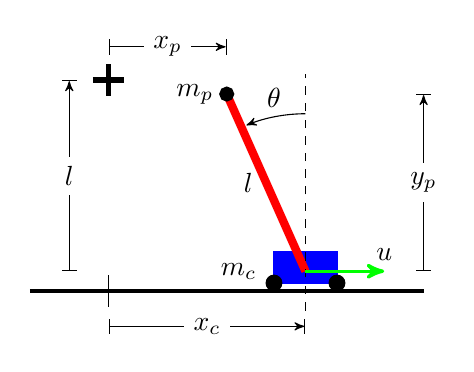
\begin{tikzpicture}
\def\xcart {2.5}     % x-position of center of the cart
\def\ycart {0.25}  % y-position of center of the cart
\def\wheelR {0.1} % Radius of wheels
\def\cartW  {0.8} % Width of the cart
\def\cartH {0.4}  % Heigt of the cart
\def\ang {22}     % Angle theta
\def\xtipR {-1}   % Relative x-Position of tip of the pendululum with respect to center of cart
\def\ytipR {2.25} % Relative x-Position of tip of the pendululum with respect to center of cart
\def\goallen {0.2} % Goal offset lengths
\def\pendlen {2.427} % = \ytipR/cos(\pendulumangle)
%\definecolor{brown}{rgb}{0.858, 0.188, 0.478}
% rail:
 % \draw[draw=none,pattern=north east lines,pattern color=lightgray](-3,0) rectangle (5,-0.2);
  \draw[draw=black,ultra thick] (-1,0) -- (4,0);
 % cart:
 \draw[draw=blue,fill=blue] (\xcart-\cartW/2,\wheelR) rectangle (\xcart+\cartW/2,\wheelR+\cartH);
 \draw[draw=black,fill=black] (\xcart-\cartW/2,\wheelR) circle (\wheelR cm);
 \draw[draw=black,fill=black] (\xcart+\cartW/2,\wheelR) circle (\wheelR cm);
 \node[anchor=east] at (\xcart-\cartW+0.3,\ycart) {$m_c$};
% pole:
 \draw[draw=red, line width = 3pt] (\xcart,\ycart) -- (\xcart+\xtipR,\ycart+\ytipR)node[anchor= east] {$m_p$}  node[anchor= east, midway]  {$l$};
 \draw[draw=black, line width = 3pt] (\xcart+\xtipR,\ycart+\ytipR) circle (0.04cm);
%% geometry:
 \draw[draw=black, dashed] (\xcart,\ycart-0.5) -- (\xcart,\ycart+2.5);
 \draw[draw=black] (0,-.2) -- (0,.2);
 \draw [->] ([shift=(90:2)]\xcart,\ycart)  arc (90:90+\ang:2) node[xshift=0.35cm, yshift=0.35cm] {$\pendulumangle$};
 \draw [|->|,draw=black] (0,-0.45) -- (\xcart,-0.45) node[fill=white, midway] {$x_c$};
 \draw[|->|,draw=black] (\xcart+\xtipR+2.5,\ycart) -- (\xcart+\xtipR+2.5,\ycart+\ytipR) node[fill=white, midway]  {$y_p$};
 \draw[|->|,draw=black] (0,\ycart+\ytipR+0.6) -- (\xcart+ \xtipR,\ycart+\ytipR+0.6) node[fill=white, midway]  {$x_p$};
%% goal
 \draw[draw=black, line width = 2pt] (0,\pendlen+\ycart-\goallen) -- (0,\pendlen+\ycart+\goallen);
 \draw[draw=black, line width = 2pt] (-\goallen,\pendlen+\ycart) -- (\goallen,\pendlen+\ycart);
 \draw[|->|,draw=black] (-0.5,\ycart) -- (-0.5,\pendlen+\ycart) node[fill=white, midway] {$l$};
%% force:
 \draw[very thick,draw=green,->]  (\xcart,\ycart) -- (\xcart +1,\ycart) node[anchor=south]  {$u$};
\end{tikzpicture}
\caption{\textbf{The cartpole swing-up task.}
A pendulum of length $l$ is attached to a cart by a frictionless pivot.
The cart has mass $m_c$ and position $x_c$.
The pendulum's endpoint has mass $m_p$ and position $(x_p,y_p)$, with angle $\pendulumangle$ from vertical.
The cart begins at position $x_c=0$ and pendulum hanging down: $\pendulumangle=\pi$.
The goal is to accelerate the cart by applying horizontal force $u_t$ at each timestep $t$
to invert then stabilise the pendulum's endpoint at the goal (black cross),
i.e.\ to maintain $x_c=0$ and $\pendulumangle=0$.
}
\label{fig:cartpole} % must come after caption
\end{figure}

We compare four algorithms:
1) PILCO by \citet{pilco} as a baseline (unfiltered execution, and unfiltered full-prediction);
2) the method by \citet{dallaire2009} (filtered execution, and filtered MAP-prediction);
3) the method by \citet{deisenroth2013} (filtered execution, and unfiltered full-prediction);
and lastly
4) our method (filtered execution, and filtered full-prediction).
For clear comparison
we opted for a tightly controlled experiment.
We control for data and dynamics models,
i.e.\ each algorithm has access to the exact same data and exact same dynamics model.
The reason is to
%avoid the possibility of one algorithm getting `lucky' and discovering more useful data
%than another
%due to randomised observations and initialisation during execution.
eliminate variance in performance caused by different algorithms choosing different actions.
We generate a single dataset by running the baseline PILCO algorithm
for 11 episodes (totalling 22 seconds of system interaction). % todofinal: verify still correct?
%Thus, each algorithm has access to the same transition dataset, and same dynamics model
%(generated by baseline \cite{pilco} algorithm).
The independent variables of our experiment are
1) the method of system prediction and
2) the method of system execution.
We then optimise each policy from the same initialisation
using their respective prediction methods.
Finally, we measure and compare their performances
in both prediction and execution.

\section{Results and Analysis}\label{sec:result-and-analysis}

\subsection{Predictive Performance}
We now compare algorithm performance, both predictive (Figure~\ref{fig:simulation-results})
and % from
empirical % execution
(Figure~\ref{fig:empirical-results}).
%
First, we analyse predictive costs per timestep (Figure~\ref{fig:simulation-results}).
Since predictions are probabilistic,
the costs have distributions, % approximated as Gaussian.
with the exception of \citet{dallaire2009} which predicts MAP trajectories
and therefore has deterministic cost.
Even though we plot distributed costs,
policies are optimised w.r.t.\ expected total cost only.
%
Using the same dynamics,
the different prediction methods optimise different policies
(with the exception of \citet{pilco} and \citet{deisenroth2013},
whose prediction methods are identical).
During the first 10 timesteps, we note % todofinal
identical performance with maximum cost
due to the non-zero time required physically swing the pendulum up
near the goal.
Performances thereafter diverge.
Since we predict w.r.t.\ a filtering process,
less noise is predicted to be injected into the policy,
and the optimiser can thus afford higher gain parameters w.r.t.\ the pole at balance point.
If we linearise our policy around the goal point,
our policy has a gain of -81.7N/rad w.r.t.\ pendulum angle,
a larger-magnitude than both Deisenroth method gains of -39.1N/rad
(negative values refer to \textit{left} forces in Figure~\ref{fig:cartpole}).
Being afforded higher gains
our policy is more reactive and more likely to catch a falling pendulum.
% Because it knows of this advantage, it predicts a greater advantage than both Deisenroth's methods.
Finally,
we note \citet{dallaire2009} predict very high performance.
Without balancing the costs across multiple possible trajectories,
the method instead optimises a sequence of deterministic states to near perfection.

\subsection{Empirical Performance}
%\paragraph{Execution:}
To compare the predictive results against the empirical,
we used 100 executions of each algorithm (Figure~\ref{fig:empirical-results}).
First, we notice a stark difference between predictive and executed performances from \citet{dallaire2009},
due to neglecting model uncertainty, suffering model bias.
In contrast, the other methods consider uncertainty and have relatively unbiased predictions,
judging by the similarity between predictive-vs-empirical performances.
Deisenroth's methods, which differ only in execution,
illustrate that filtering during execution-only can be better than no filtering at all.
However, the major benefit comes when
the policy is evaluated from multi-step predictions of a filtered system.
Opposed to \citet{deisenroth2013},
our method's predictions reflect reality closer
because we both predict and execute system trajectories
using closed loop filtering control. % TODO: reword

To test statistical significance of empirical cost differences given 100 executions,
we use a Wilcoxon rank-sum test at each time step.
Excluding time steps ranging $t=[0,29]$ (whose costs are similar),
the minimum $z$-score over timesteps $t=[30,60]$
that our method has superior average-cost than each other methods follows:
Deisenroth 2011 $\min(z) = 4.99$,
Dallaire 2009's $\min(z) = 8.08$,
Deisenroth 2012's $\min(z) = 3.51$.
Since the minimum $\min(z) = 3.51$, we have $p>99.9\%$ certainty our method's
average empirical cost is superior than each other method.
% TODO: clean above


\subsection{Training Time Complexity}
Training the GP dynamics model involved $N=660$ data, $M=50$ inducing points under a sparse GP FITC
$P=100$ policy RBF centroids, $D=4$ state dimensions, $F=1$ action dimensions, and $T=60$ timestep horizon.
To train the dynamics model scales $\mathcal{O}(DNM^2)$.
Policy optimisation (with 300 steps,
each of which require trajectory prediction with gradients) is the most intense part:
our method and both Deisenroth's methods scale $\mathcal{O}(M^2 D^2 (D+F)^2 T + P^2 D^2 F^2 T)$,
whilst Dallaire's only scales $\mathcal{O}(MD(D+F)T + PDFT)$.
Worst case we require $M = \mathcal{O}(\exp(D+F))$ inducing points to capture dynamics, the average case is unknown.
Total training time was four hours to train the original PILCO method
with an additional one hour to re-optimise the policy.

\section{Conclusion and Future Work}\label{sec:conclusions}

\newcommand{\graphscale}{0.89}
\newcommand{\xmins}{0}
\newcommand{\horizon}{60} % 30 45 60
\newcommand{\ymins}{0}
\newcommand{\ymaxs}{1}
\newcommand{\xticks}{0,10,20,30,40,50,60}
\newcommand{\xlabels}{Timestep}
\newcommand{\ylabels}{Cost}
\newcommand{\legends}{legend entries={
(NFexe | NFsim),
Dallaire (BFexe | BFMAPsim),
Deisenroth (BFexe | NFsim),
CtrlBF (BFexe | BFsim)},}
\newcommand{\legendstyle}{legend style={at={(0.955,0.96)},anchor=north east}}

% pg 195 and pg 198 of pgfplots manual:
\pgfplotscreateplotcyclelist{rowan}{%
blue,every mark/.append style={fill=blue!80!black},mark=*\\%
red,every mark/.append style={fill=red!80!black},mark=square*\\%
yellow!55!black,every mark/.append style={fill=yellow!75!black},mark=triangle*\\%
black,mark=x\\%
}

\begin{figure}[t]
\centering
\begin{minipage}[t]{0.52\textwidth}\hspace{-3mm}
%\vspace{-2mm}
% Preamble: \pgfplotsset{width=7cm,compat=1.13}
\begin{tikzpicture}[scale=\graphscale]
\begin{axis}[
xlabel=\xlabels,
ylabel=\ylabels, ylabel absolute, ylabel style={yshift=-4mm},
%enlarge x limits=0,
xtick={\xticks},
xmin=\xmins,
xmax=\horizon,
ymin=\ymins,
ymax=\ymaxs,
% \legends,
legend entries={\small{Deisenroth 2011},
\small{Dallaire 2009},
\small{Deisenroth 2012},
\small{Our Method}},
%legend entries={\cite{pilco},\cite{dallaire2009},\cite{deisenroth2013},Our Method},
\legendstyle,
legend cell align=left,
cycle list name=rowan,
]
\input{\graphA}
\end{axis}
\end{tikzpicture}
\caption{\textbf{Predictive costs per timestep.}
The error bars show $\pm1$ standard deviation.
Each algorithm has access to the same data set
(generated by baseline Deisenroth 2011) and dynamics model.
Algorithms differ in their multi-step prediction methods
(except Deisenroth's algorithms whose predictions overlap).
}
\label{fig:simulation-results} % must come after caption
%\end{figure}
\end{minipage}
% http://tex.stackexchange.com/questions/47345/specify-the-step-of-pgfplots-axis
% http://pgfplots.sourceforge.net/pgfplots.pdf around pg 300.
\hspace{3mm}
%\begin{figure}[t]
\begin{minipage}[t]{0.43\textwidth}\hspace{-8mm}
%\vspace{-2mm}
% Preamble: \pgfplotsset{width=7cm,compat=1.13}
\begin{tikzpicture}[scale=\graphscale]
\begin{axis}[
xlabel=\xlabels,
%ylabel=\ylabels, ylabel absolute, ylabel style={yshift=-0.15cm},
xtick={\xticks},
xmin=\xmins,
xmax=\horizon,
ymin=\ymins,
ymax=\ymaxs,
% \legends,
%legend entries={\cite{pilco},\cite{dallaire2009},\cite{deisenroth2013},Our Method},
\legendstyle,
legend cell align=left,
cycle list name=rowan,
]
\input{\graphB}
\end{axis}
\end{tikzpicture}
\caption{%Costs per timestep from system execution.
\textbf{Empirical costs per timestep}.
We generate empirical cost distributions from 100 executions per algorithm.
%the same 100 from Figure~\ref{fig:simulation-results}.
Error bars show $\pm1$ standard deviation.
The plot colours and shapes correspond to the legend in Figure~\ref{fig:simulation-results}.
}
\label{fig:empirical-results} % must come after caption
%\vspace{-4mm}
\end{minipage}
\end{figure}

In this paper,
we extended the original PILCO algorithm \cite{pilco} to filter observations,
both during system execution and multi-step probabilistic prediction required for policy evaluation.
The extended framework enables learning in \textit{partially-observed} environments (POMDPs)
whilst retaining PILCO's data-efficiency property.
We demonstrated successful application to a benchmark control problem,
the noisily-observed cartpole swing-up.
Our algorithm %retained its data-efficiency properties,
learned a good policy under significant observation noise in less than 30 seconds of system interaction. % todofinal: still true?
%This was possible with the combination of a filter using probabilistic dynamics model
%used to propagate dynamics uncertainty all the way throughout system-prediction up until the horizon.
Importantly, our algorithm evaluates policies with predictions that are faithful to reality.
We predict w.r.t.\ closed loop filtered control precisely because we execute closed loop filtered control,
unlike other RL algorithms. % in the literature.

We showed experimentally that \textit{faithful} and \textit{probabilistic}
predictions give greater performance gains than otherwise.
For clear comparison we constrained each algorithm to use the same dynamics dataset
rather than each interacting with the system to generate their own.
Thus, we cannot currently claim superior data-collection abilities of our method,
only superior data-usage.
In future work we wish to relax this experimental constraint, % TODO: Yarin say mention we really don't want to do this for future work etc, we want to say the previous was a typical run.
to test a difference in data-collection abilities.
However, the extra variance in empirical performance
(caused by selection of different data)
means a much larger number of experiments
will be required to detect if such \textit{additional} performance gains exist.

Several more challenges remain for future work.
Firstly the assumption of zero variance of the belief-variance could be relaxed.
A relaxation allows distributed trajectories to more accurately
consider belief states having various degrees of certainty (belief-variance).
E.g. system trajectories have larger belief-variance when passing though
data-sparse regions of state-space,
and smaller belief-variance in data-dense regions.
Secondly, the policy could be a function of the full belief distribution (mean and variance)
rather than just the mean. Such flexibility could help the policy make more `cautious' actions when more uncertain about the state.
Thirdly, the framework could be extended to active learning.
Currently, the framework is a passive learner,
greedily optimising the total cost-means
and ignoring cost-variance information which could otherwise better inform exploration,
increasing data-efficiency further.
%closer to the Bayes-optimal policy.

\newpage
\bibliographystyle{apalike}
\bibliography{nips2016_filtering}

\newpage
\appendix

\section{Gradients for Policy Improvement} \label{sec:app-gradients} % TODO: this isn't finished?
Let $\uw(\cdot)$ be the `unwrap operator'
that reshapes matrices columnwise into vectors.
We define a Markov filtered-system from the belief's parameters:
%$\now{S}=[\now{\BJ}^\top,\uw(\pno{V})^\top]^\top % TODO?: get rid of S, just use B.
\smash{$\now{S}=[\pno{\BM}^\top,\;\uw(\pno{V})^\top]^\top$}.
To predict system evolution, the state distribution is defined: % 111
\begin{equation}
p(\now{S})
\sim\N\left(\now{\mu}^s=\begin{bmatrix} \pno{\mu}^\bm \\ \uw(\pne{V}) \end{bmatrix}, % TODO: \uw(\pne{\bar V}): \bar V was introduces in appendix not here...?
\;\;\now{\Sigma}^s=\begin{bmatrix} \pno{\Sigma}^\bm &0 \\0 &0\end{bmatrix}\right).
\end{equation}
To compute policy gradient $\der J/\der\policyparams$
we first require $\der \now{\expcost} / \der \policyparams$:
%at each time $t$ to chain together,
%and thus $\der p(\now{S}) / \der \policyparams$,
\begin{eqnarray}\frac{\der \now{\expcost}}{\der\theta}&\;\;=\;\;&
\frac{\der\now{\expcost}}{\der p(\now{S})} \frac{\der p(\now{S})}{\der \theta}\nnn
% &\;=\;& \frac{\der\now{\expcost}}{\partial \mu_\bj} \frac{\partial \mu_\bj}{\der \theta} +
% \frac{\der\now{\expcost}}{\partial \Sigma_\bj} \frac{\partial \Sigma_\bj}{\der \theta} +
% \frac{\der\now{\expcost}}{\partial \pno{V}} \frac{\partial \pno{V}}{\der \theta} % TODO is \pno correct?
% &\;=\;&
&\;\;=\;\;&\frac{\der\now{\expcost}}{\partial \now{\mu}^s} \frac{\partial \now{\mu}^s}{\der \theta} +
\frac{\der\now{\expcost}}{\partial \now{\Sigma}^s} \frac{\partial \now{\Sigma}^s}{\der \theta},\quad\quad\text{and}\\
%
\frac{\der p(\new{S})}{\der\theta}&\;=\;&\frac{\der p(\new{S})}{\der p(\now{S})}
\frac{\der p(\now{S})}{\der\theta} + \frac{\partial p(\new{S})}{\partial\theta}.
\end{eqnarray}

Application of the chain rule backwards from the state distribution at the horizon $S_T$,
to $S_t$ at arbitrary time $t$,
is analogous to that detailed in
PILCO \cite{pilco},
% where we use $\now{\BJ}$, $\mu_{\bj}$ and $\Sigma_{\bj}$ in the place of
% $\now{x}$, $\now{\mu}$ and $\now{\Sigma}$ respectively,
% and including one extra chain term $\pno{V}$.
where we use $\now{S}$, $\now{\mu}^s$ and $\now{\Sigma}^s$ in the place of
$\now{x}$, $\now{\mu}$ and $\now{\Sigma}$ respectively.

\section{Identities for Gaussian Process
Prediction with Hierarchical Uncertain Inputs}

The two functions
\begin{equation}
\begin{split}
q(x,x',\Lambda,V)\;\triangleq&\;|\Lambda^{-1}V+I|^{-1/2}\exp\big(-\tfrac{1}{2}(x-x')[\Lambda+V]^{-1}(x-x')\big),\\
Q(x,x',\Lambda_a,\Lambda_b,V, \mu, \Sigma)\;\triangleq&\;
c_1\exp\big(-\tfrac{1}{2}(x-x')^\top[\Lambda_a+\Lambda_b+2V]^{-1}(x-x')\big)\\
&\times\,\exp\big(-\tfrac{1}{2}(z-\mu)^\top\big[\big((\Lambda_a+V)^{-1}+(\Lambda_b+V)^{-1}\big)^{-1}+\Sigma\big]^{-1}(z-\mu)\big),\\
=&\;c_2\,q(x,\mu,\Lambda_a,V)\,q(\mu,x'\Lambda_b,V)\\
&\times\,\exp\big(\tfrac{1}{2}{\bf
  r}^\top\big[(\Lambda_a+V)^{-1}+(\Lambda_b+V)^{-1}+\Sigma^{-1}\big]^{-1}{\bf r}\big),\\
\text{where}&\left\{\begin{array}{l}
z\;=\;(\Lambda_b+V)(\Lambda_a+\Lambda_b+2V)^{-1}x+(\Lambda_a+V)(\Lambda_a+\Lambda_b+2V)^{-1}x'\\
{\bf r}\;=\;(\Lambda_a+V)^{-1}(x-\mu)+(\Lambda_b+V)^{-1}(x'-\mu)\\
c_1\;=\;\big|(\Lambda_a+V)(\Lambda_b+V)+(\Lambda_a+\Lambda_b+2V)\Sigma\big|^{-1/2}\big|\Lambda_a\Lambda_b\big|^{1/2}\;\\
c_2\;=\;\big|\big((\Lambda_a+V)^{-1}+(\Lambda_b+V)^{-1}\big)\Sigma+I\big|^{-1/2},\end{array}\right.
\end{split}
\end{equation}
have the following Gaussian integrals
\begin{equation}
\begin{split}
\int q(x,t,\Lambda,V){\cal N}(t|\mu,\Sigma)dt\;=&\;q(x,\mu,\Lambda,\Sigma+V),\\
\int q(x,t,\Lambda_a,V)\,q(t,x',\Lambda_b,V)\,{\cal
  N}(t|\mu,\Sigma)dt\;=&\;Q(x,x',\Lambda_a,\Lambda_b,V,\mu,\Sigma),\\
\int Q(x,x',\Lambda_a,\Lambda_b,0,\mu,V){\cal N}(\mu|\bfm,\Sigma)d\mu\;=&\;Q(x,x',\Lambda_a,\Lambda_b,0,\bfm,\Sigma+V).
\end{split}
\end{equation}
%
We want to model data with $E$ output coordinates, and use separate
combinations of linear models and GPs to make predictions,
$a=1,\ldots,E$:
\[
f_a(x^*)\;=\;f_a^*\;\sim\;{\cal N}\big(\theta_a^\top x^*+k_a(x^*,\bfx)\beta_a,\;
k_a(x^*,x^*)-k_a(x^*,\bfx)(K_a+\Sigma_\varepsilon^a)^{-1}k_a(\bfx,x^*)\big),
\]
where the $E$ squared exponential covariance functions are
\begin{equation}
k_a(x,x')\;=\;s_a^2q(x, x',\Lambda_a,0), \text{\ \ where\ \ }a=1,\ldots,E,
\end{equation}
and $s_a^2$ are the signal variances and $\Lambda_a$ is a diagonal
matrix of squared length scales for GP number $a$. The noise variances
are $\Sigma_\varepsilon^a$. The inputs are $\bfx$ and the outputs
$y_a$ and we define $\beta_a=(K_a+\Sigma_\varepsilon^a)^{-1}(y_a-\theta_a^\top\bfx)$,
where $K_a$ is the Gram matrix.

\subsection{Derivatives}

% q function partial derivatives
For symmetric $\Lambda$ and $V$ and $\Sigma$:
\begin{equation}
\begin{split}
\frac{\partial \ln q(x,x',\Lambda,V)}{\partial x}
\;=&\; -(\Lambda+V)\inv (x-x') = -(\Lambda\inv V+I)\inv\Lambda\inv (x-x') \\
\frac{\partial \ln q(x,x',\Lambda,V)}{\partial x'}
\;=&\; (\Lambda+V)\inv (x-x') \\
\frac{\partial \ln q(x,x',\Lambda,V)}{\partial V}
\;=&\; -\frac{1}{2}(\Lambda+V)\inv + \frac{1}{2}(\Lambda+V)\inv(x-x')(x-x')^\top(\Lambda+V)\inv
\end{split}
\end{equation}

% Q function partial derivatives
Let
$L=(\Lambda_a+V)\inv+(\Lambda_b+V)\inv$,
$R=\Sigma L+I$,
$Y=R\inv \Sigma=\big[L+\Sigma\inv\big]\inv$,
$T: X \rightarrow XX^\top$:
\begin{equation}
\begin{split}
&\partial Q(x,x',\Lambda_a,\Lambda_b,V, \mu, \Sigma)
\;=\; Q \circ \partial \Big( \ln c_2 + \ln q(x,\mu,\Lambda_a,V) +
\ln q(\mu,x'\Lambda_b,V) +
\frac{1}{2} y^\top Y y \Big) \\
% \mu:
&\frac{1}{2}\frac{\partial \, y^\top Y y}{\partial \mu} =
y^\top  Y \frac{\partial y}{\partial \mu} = -y^\top YL \\
% \Sigma:
& \frac{\partial \ln c_2}{\partial \Sigma} = -\frac{1}{2}\frac{\partial \ln |L\Sigma +I|}{\partial\Sigma} =
-\frac{1}{2}L^\top(L \Sigma+I)\invt = -\frac{1}{2}LR\inv \\
&\frac{\partial \, y^\top Y y}{\partial \Sigma} =
\Sigma\invt Y^\top yy^\top  Y^\top\Sigma\invt =
T(R\invt y) \\
% V:
& \frac{\partial \ln c_2}{\partial V} = -\frac{1}{2}\frac{\partial \ln |L\Sigma +I|}{\partial V} =
-\frac{1}{2}\frac{\partial \ln |\sum_i \big[(\Lambda_i+V)\inv\big]\Sigma +I|}{\partial V} \\
&\hspace{1.0cm} = \frac{1}{2} \sum_i \Big[ (\Lambda_i+V)\invt \Big(\sum_j \big[(\Lambda_j+V)\inv\big]\Sigma +I\Big)\invt \Sigma^\top (\Lambda_i+V)\invt \Big]
\\
&\hspace{1.0cm} =
\frac{1}{2} \sum_i \Big[ (\Lambda_i+V)\inv Y (\Lambda_i+V)\inv \Big]
\\
%
&\frac{\partial \, y^\top Y y}{\partial V} =
y^\top \frac{\partial \,  Y}{\partial V} y +
 \frac{\partial y^\top}{\partial V} Y y +  y^\top Y \frac{\partial y}{\partial V}
\;\;\; = \;\;\;  \sum_i \Big[ (\Lambda_i+V)\inv Y^\top yy^\top Y^\top (\Lambda_i+V)\inv \Big] \\
&\hspace{3.0cm}
- \sum_i \Big[ (\Lambda_i+V)\inv (x_{n_i}-\mu) (Y y)^\top (\Lambda_i+V)\inv \Big] \\
&\hspace{3.0cm} - \sum_i \Big[ (\Lambda_i+V)\inv (y^\top Y)^\top (x_{n_i}-\mu)^\top (\Lambda_i+V)\inv \Big] \\
&\hspace{1.0cm} =   \sum_i \Big[ T \Big( (\Lambda_i+V)\inv (Yy - (x_{n_i}-\mu)) \Big) -
T \Big( (\Lambda_i+V)\inv (x_{n_i}-\mu) \Big) \Big]
\end{split}
\end{equation}

\newpage
\section{Dynamics Predictions in System-Execution} \label{sec:app-instantiation-prediction} % Instantiated-System Predictions
% from \subsection{System Prediction} % TODO: the way I have defined the expectation over function f, needs to be replicated in the GPH derivations in the appendix for consistency.
% 222
Here we specify the predictive distribution $p(\pne{b})$,
whose moments are equal to the moments from dynamics model output $\fb$ with uncertain input
$\unot{b}\sim\N(\unot{\bm},\unot{V})$ similar to \citet{pilco}.
%
Consider making predictions from $a=1,\ldots,E$ GPs at $\unot{b}$ with specification
%\begin{equation}
$p(\unot{b})\;\sim\;{\cal N}(\unot{\bm}, \unot{V})$.
%\end{equation}
%
We have the following expressions for the predictive mean, variances
and input-output covariances using the law of iterated expectations and variances:

\begin{eqnarray}
%\begin{split}
\pne{b}&\sim&\N(\pne{\bm},\pne{V}),\label{eq:pneb}\\
\pne{\bm}^a&=&\E_{\unot{b}}[\fb^a(\unot{b})]\nnn
&=&\int\big(s_a^2\beta_a^\top q(x_i,\unot{b},\Lambda_a,0)+\gplinear_a^\top\unot{b}\big){\cal N}(\unot{b};\unot{\bm},\unot{V})d\unot{b}\nnn
&=&s_a^2\beta_a^\top q^a+\gplinear_a^\top\unot{\bm},\label{eq:pnez}\\ % TODO: decide a above or below on q's betas??
C_a
&\doteq&\unot{V}\inv\C_{\unot{b}}[\unot{b},\fb^a(\unot{b})-\gplinear_a^\top\unot{b}],\nnn
&=&\unot{V}\inv\int(\unot{b}-\unot{\bm})s^2_a\beta_a^\top q(\text{x},\unot{b},\Lambda_a,0)\N(\unot{b};\unot{\bm},\unot{V})d\unot{b}\nnn
&=&s^2_a(\Lambda_a+\unot{V})^{-1}(\text{x}-\unot{\bm})\beta_aq^a,\label{eq:pneC}\\
\pne{V}^{ab}
&=&\C_{\unot{b}}\left[\fb^a(\unot{b}),\;\fb^b(\unot{b})\right]\nnn
%
&=&\C_{\unot{b}}\left[\E_f[\fb^a(\unot{b}), \E_f[\fb^b(\unot{b})\right]+\E_{\unot{b}}\left[\C_f[\fb^a(\unot{b}),\;\fb^b(\unot{b})]\right]\nnn
&=&\C_{\unot{b}}\left[s_a^2\beta_a^\top q(\text{x},\unot{b},\Lambda_a,0)+\gplinear_a^\top \unot{b},\;\;s_b^2\beta_b^\top q(\text{x},\unot{b},\Lambda_b,0)+\gplinear_b^\top \unot{b}\right]+\nnn
&&
\delta_{ab}\E[s_a^2-k_a(\unot{b},\text{x})(K_a+\Sigma_\varepsilon^a)^{-1}k_a(\text{x},\unot{b})]\label{eq:v}\nnn
%
&=& s_a^2s_b^2\big[\beta_a^\top ( Q^{ab}\!-\!q^a q^{b\top})\beta_b+\nnn
 &&\delta_{ab}\big(s_a^{-2}\!-\!\operatorname{tr}((K_a+\Sigma_\varepsilon^a)^{-1} Q^{aa})\big)\big]+
 C_a^\top\unot{V} \gplinear_b + \gplinear_a^\top\unot{V} C_b + \gplinear_a^\top\unot{V} \gplinear_b,\label{eq:pneV}
\end{eqnarray}
where
\begin{eqnarray}
q^a_i&=&q\big(\text{x}_i,\unot{\bm},\Lambda_a,\unot{V}\big),\nnn
Q^{ab}_{ij}&=&Q\big(\text{x}_i,\text{x}_j,\Lambda_a,\Lambda_b,0,\unot{\bm},\unot{V}\big),\nnn
%&q(\text{x}_i,\mu,\Lambda,V)\doteq|\Lambda^{-1}V+I|^{-1/2}\exp\big(-\tfrac{1}{2}(\text{x}_i-\mu)[\Lambda+V]^{-1}(\text{x}_i-\mu)\big),\nnn
%&Q(x_i,x_j,\Lambda_a,\Lambda_b,V, \mu, \Sigma)\;\doteq\;c\,q(x_i,\mu,\Lambda_a,V)\,q(x_j,\mu,\Lambda_b,V)\nnn
%&\newlinetimesdist\exp\big(\tfrac{1}{2}\text{z}_{ij}^\top\big[(\Lambda_a+V)^{-1}+(\Lambda_b+V)^{-1}+\Sigma^{-1}\big]^{-1}\text{z}_{ij}\big),\\
%&Q(\text{x}_i,\text{x}_j,\Lambda_a,\Lambda_b,V, \mu, \Sigma)\doteq|R|^{-1/2}
%q(\text{x}_i,\mu,\Lambda_a,V)\,q(\text{x}_j,\mu,\Lambda_b,V)
%\exp\big(\tfrac{1}{2}\text{z}_{ij}^\top R^{-1}\Sigma\text{z}_{ij}\big),\nnn
%&R=\Sigma\big((\Lambda_a+V)^{-1}\!+\!(\Lambda_b+V)^{-1}\big)+I,\quad\quad
%&c\;=\;\big|\big((\Lambda_a+V)^{-1}+(\Lambda_b+V)^{-1}\big)\Sigma+I\big|^{-1/2},\\
%\text{z}_{ij}=(\Lambda_a+V)^{-1}(x_i\!-\!\mu)+(\Lambda_b+V)^{-1}(x_j\!-\!\mu),\nnn
\beta_a&=&(K_a+\Sigma^{\epsilon,a})^{-1}(y_a-\gplinear_a^\top\text{x}),\nn
\end{eqnarray}
and training inputs are $\text{x}$,
outputs are $y_a$ (determined by the `Direct method'),
$K_a$ is a Gram matrix. % TODO: define here or in paper if now used in paper?
%and the GP linear mean function has weight-vector $\gplinear_a\in\mathbb{R}^D$.

\section{Dynamics Predictions in System-Prediction} \label{sec:app-simulation-prediction} % Simulated-System Predictions

Here we describe the prediction formulae for the random belief state in system-prediction.
%Instead of making relative state predictions with a zero mean function,
%we make absolute state prediction with a linear mean function, with weights $\gplinear$.
We again note, during execution, our belief distribution is specified by certain parameters,
$\uno{b}\sim\N(\uno{\bm},\uno{V})$.
By contrast, during system prediction, % TODO: cut down - I've described this before.
our belief distribution is specified by an uncertain belief-mean and certain belief-variance:
\smash{$\uno{B}\sim\N(\uno{\BM},\uno{V})\sim\N(\N(\uno{\mu}^m,\uno{\Sigma}^m),\uno{\bar V})$},
where we assumed a delta distribution on $\uno{\bar V}$ for mathematical simplicity,
i.e.\ $\uw(\uno{V})\sim\N(\uw(\uno{\bar V}),0)$.
Therefore we conduct GP prediction given hierarchically-uncertain inputs,
outlining each output moment below. % TODO: reword.
%$\uno{B}\sim\N(\uno{\BM},\uno{V})\sim\N(\N(\uno{\mu}^m,\uno{\Sigma}^m),\N(\uno{\bar V},0))$.
%
I.e. consider making predictions from $a=1,\ldots,E$ GPs at $\uno{B}$ with \emph{hierarchical} specification
\begin{equation}
p(\uno{B})\;\sim\;\N(\uno{\BM},\uno{V}),\text{\ \ and\ \ }\uno{\BM}\;\sim\;\N(\uno{\mu}^m,\uno{\Sigma}^m),
\end{equation}
%
or equivalently the joint
%
\begin{equation}
p\big(\Big[\!\begin{array}{c}\uno{B}\\
  \uno{\BM}\end{array}\!\Big]\big)\;\sim\;{\cal
  N}\big(\Big[\!\begin{array}{c}\uno{\mu}^m\\
  \uno{\mu}^m\end{array}\!\Big],\Big[\!\begin{array}{cc}\uno{\Sigma}^m+\uno{\bar V}&\uno{\Sigma}^m\\ \uno{\Sigma}^m&\uno{\Sigma}^m\end{array}\!\Big]\big).
\end{equation}





\paragraph{Mean of the Belief-Mean:}
dynamics prediction uses input
$\unot{\BM}\sim \N(\unotMbm,\unotSbm)$,
which is jointly distributed according to Eq.~\ref{eq:postA}.
Using the belief-mean $\pne{\bm}^a$ definition (Eq.~\ref{eq:pnez}),
\begin{eqnarray}
\pne{\mu}^{\bm,a}
&\;=\;&\E_{\unot{\BM}}[\pne{\BM}^a]\nnn
&\;=\;&\int \pne{\BM}^a \N(\unot{\BM};\unotMbm,\unotSbm)\der\unot{\BM},\nnn
&\;=\;&s_a^2\beta_a^\top\int q(\text{x},\unot{\BM},\Lambda_a,V){\cal N}(\unot{\BM};\unotMbm,\unotSbm)d\unot{\BM}+\gplinear_a^\top \unotMbm \nnn
&\;=\;&s_a^2\beta_a^\top \hat q^a +\gplinear_a^\top \unotMbm,\\
\hat q^a_i&\;=\;&q\Big(x_i,\unotMbm,\Lambda_a,\unotSbm+\unot{V}\Big).
\end{eqnarray}

\paragraph{Input-Output Covariance:}
the expected input-output covariance belief term (Eq.~\ref{eq:pneC})
(equivalent to the input-output covariance of the belief-mean) is:
\begin{eqnarray}
\hat C_a
&\;\doteq\;&\unot{V}\inv\E_{\unot{\BM}}[\C_{\uno{B}}[\unot{B},f(\unot{B})-\gplinear_a^\top \unot{\BM}]],\;\;\;\text{and similarly defined} \nnn
&\;\doteq\;&(\unotSbm)\inv\C_{\unot{\BM}}[\unot{\BM},\E_{\uno{B}}[f(\unot{B})-\gplinear_a^\top \unot{\BM}]], \nnn
%
&=&(\unotSbm)\inv\int (\unot{\BM}-\unotMbm)\E_{\uno{B}}[f(\unot{B})]{\cal N}(\unot{\BM};\unotMbm,\unotSbm)d\unot{\BM}\nnn
&=&(\unotSbm)\inv\int (\unot{\BM}-\unotMbm)\big(s^2_a\beta_a^\top
q(x_i,\unot{\BM},\Lambda_a,\unot{V}))\N(\unot{\BM};\unotMbm,\unotSbm)d\unot{\BM}\nnn
%&=&s^2_a(\Lambda_a+\unotSbm+\unot{V})^{-1}(\text{x}-\unotMbm)\beta_aq(\text{x},\unotMbm,\Lambda_a,\unotSbm+\unot{V})\nnn
%
&\;=\;&s^2_a(\Lambda_a+\unotSbm+\unot{V})^{-1}(\text{x}-\unotMbm)\beta_a\hat q^a_i.
\end{eqnarray}

\paragraph{Variance of the Belief-Mean:}
%Using the belief-mean $\pne{\bm}^a$ again,
the variance of randomised belief-mean (Eq~\ref{eq:pnez}) is:
\begin{eqnarray}
\pne{\Sigma}^{\bm,ab}
&\;=\;&\C_{\unot{\BM}}[\pne{\BM}^a,\pne{\BM}^b],\nnn
&\;=\;&\int\pne{\BM}^a \pne{\BM}^b \N(\unot{\BM}|\unotMbm,\unotSbm)\der\unot{\BM}-\mu_{\pne{\bm}}^a \mu_{\pne{\bm}}^b,\nnn
&\;=\;&s_a^2s_b^2\beta_a^\top(\hat Q^{ab}-\hat q^a \hat q^{b\top})\beta_b + \hat C_a^\top\unotSbm \gplinear_b + \gplinear_a^\top\unotSbm \hat C_b + \gplinear_a^\top\unotSbm \gplinear_b, \\
%+\hat C_a^\top\Sigma\theta_b+\theta_a^\top\Sigma\hat C_b+\theta_a^\top\Sigma\theta_b,\\
\hat Q_{ij}^{ab}&\;=\;&Q(\text{x}_i,\text{x}_j,\Lambda_a,\Lambda_b,\unot{V},\unotMbm,\unotSbm).
\end{eqnarray}

\paragraph{Mean of the Belief-Variance:}
using the belief-variance $\pne{V}^{ab}$ definition (Eq.~\ref{eq:pneV}),
\begin{eqnarray}
\pne{\bar V}^{ab}&\;=\;&\E_{\unot{\BM}}[\pne{V}^{ab}]\nnn
&\;=\;&\int \pne{V}^{ab} \N(\unot{\BM}|\unotMbm,\unotSbm)\der\unot{\BM}\nnn
&\;=\;&s_a^2s_b^2\big[\beta_a^\top (\tilde Q^{ab}-\hat Q^{ab})\beta_b+
\delta_{ab}\big(s_a^{-2}-\operatorname{tr}((K_a+\Sigma_\varepsilon^a)^{-1}\tilde
Q^{aa})\big)\big] \nnn
&&+ \hat C_a^\top\unot{V} \gplinear_b + \gplinear_a^\top\unot{V} \hat C_b + \gplinear_a^\top\unot{V} \gplinear_b, \\
% \\ %+\hat C_a^\top V\theta_b+\theta_a^\top V\hat C_b+\theta_a^\top V\theta_b,\\
\tilde Q_{ij}^{ab}&\;=\;&Q(\text{x}_i,\text{x}_j,\Lambda_a,\Lambda_b,0,\unotMbm,\unotSbm+\unot{V}).
\end{eqnarray}

% \subsection{Variance of the Belief-Variance}
% For mathematical simplicity,
% we assume no distribution over the belief variance,
% i.e.
% $\V[\uw(\pne{V})] = 0$.
% Thus,
% \begin{eqnarray}
%  \uw(\pne{V})\;\sim\;\N(\uw(\pne{\bar V}), 0).
% \end{eqnarray}

% % Undo the below for the camera-ready copy.
% % Acknowledgements should only appear in the accepted version.
% \section*{Acknowledgements}
%
% \textbf{Do not} include acknowledgements in the initial version of
% the paper submitted for blind review.
%
% If a paper is accepted, the final camera-ready version can (and
% probably should) include acknowledgements. In this case, please
% place such acknowledgements in an unnumbered section at the
% end of the paper. Typically, this will include thanks to reviewers
% who gave useful comments, to colleagues who contributed to the ideas,
% and to funding agencies and corporate sponsors that provided financial
% support.

\end{document}

